\chapter{Analisi del prodotto}
\label{cap:prodotto}

\intro{Di seguito un'analisi del prodotto Sangfor CyberCommand, con cui ho lavorato durante il mio stage.}

\section{Homepage e dashboard}

\begin{figure}[!htbp]
    \centering
    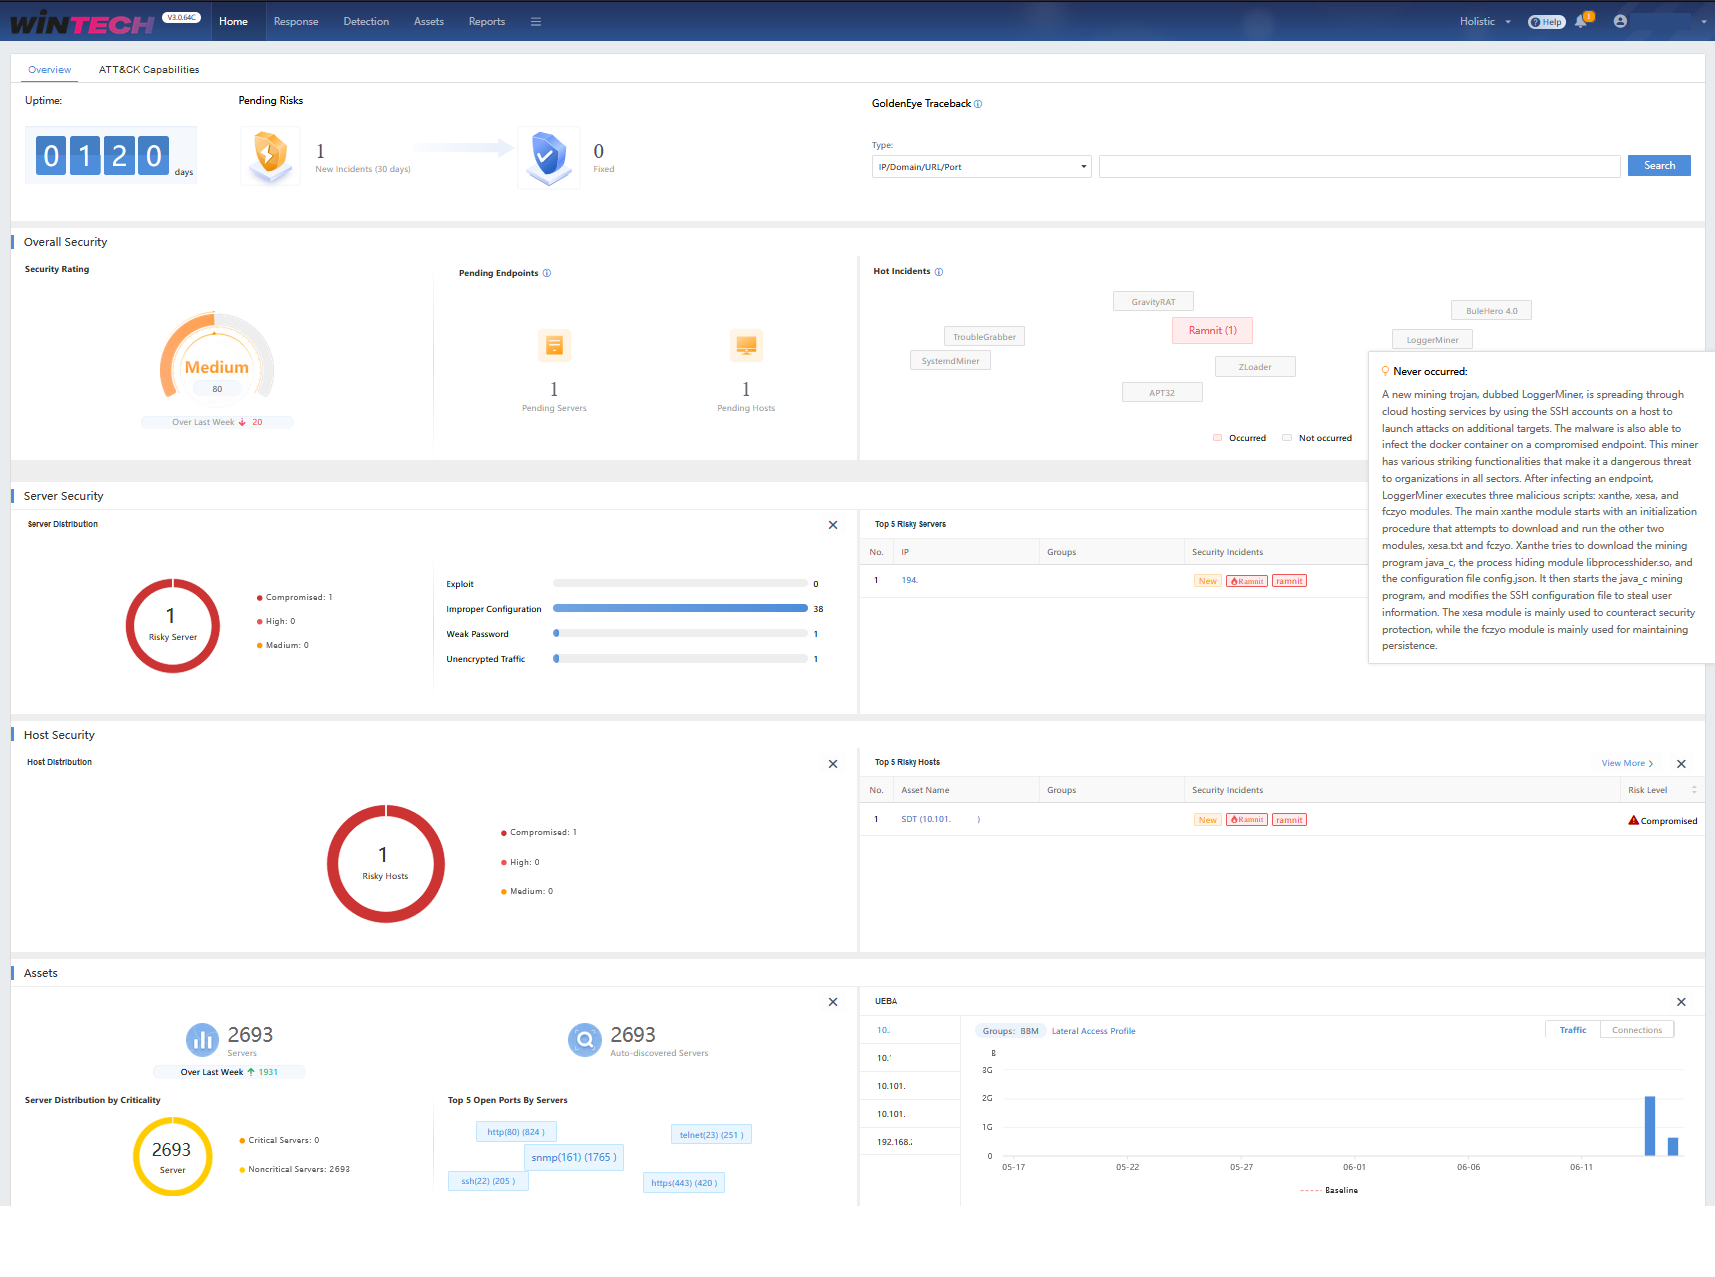
\includegraphics[width=\linewidth]{images/ndr/dashboard.png}
    \caption{Home page del CyberCommand}
    \label{fig:cc-dashboard}
\end{figure}

Analizziamo nel dettaglio i vari elementi presenti nella pagina principale del CyberCommand, mostrata in \autoref{fig:cc-dashboard}.

\begin{itemize}
    \item \emph{Menu di navigazione}: permette di navigare tra le varie pagine del sistema e di accedere alle varie funzionalità.
    \item \emph{Uptime}: mostra da quanto il sistema è in esecuzione e un contatore delle segnalazioni riscontrate.
\end{itemize}

\subsection{Overall Security}

Mostra un indice di sicurezza (\autoref{fig:cc-overall}), su una scala da 0 a 100, calcolato in base a quanti dispositivi tra \emph{server} e \emph{host} monitorati sono classificati come vulnerabili o compromessi.

\begin{figure}[!htbp]
    \centering
    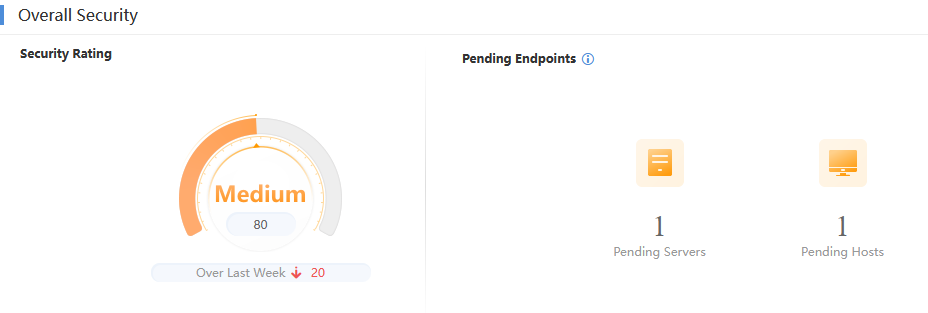
\includegraphics[width=0.8\linewidth]{images/ndr/overall-sec.png}
    \caption{Sezione di \emph{Overall Security}}
    \label{fig:cc-overall}
\end{figure}

\subsection{Server Security}
\label{sec:cc-server-sec}

Mostra la quantità di errori rilevati in un dato momento, catalogati secondo quattro categorie. In \autoref{fig:cc-server-sec} vediamo che viene mostrata in maniera molto simile alla sezione di \emph{Overall Security}. Le categorie sono:

\begin{itemize}
    \item \emph{Exploit e vulnerabilità}
    \item \emph{Weak Password}: il sistema valuta le \emph{password} che riesce a estrarre dal traffico in chiaro. Se queste non superano un controllo basato su dei requisiti minimi di sicurezza o sono contenute in una lista di \emph{password} deboli viene segnalato un errore
    \item \emph{Unencrypted Web Traffic}: se è il sistema rileva del traffico in chiaro lo segnala e propone alcune soluzioni per risolvere il problema 
    \item \emph{Improper configuration}: segnala la presenza di configurazioni note per essere rischiose, come ad esempio porte aperte che non dovrebbero esserlo
\end{itemize}

\begin{figure}[!htbp]
    \centering
    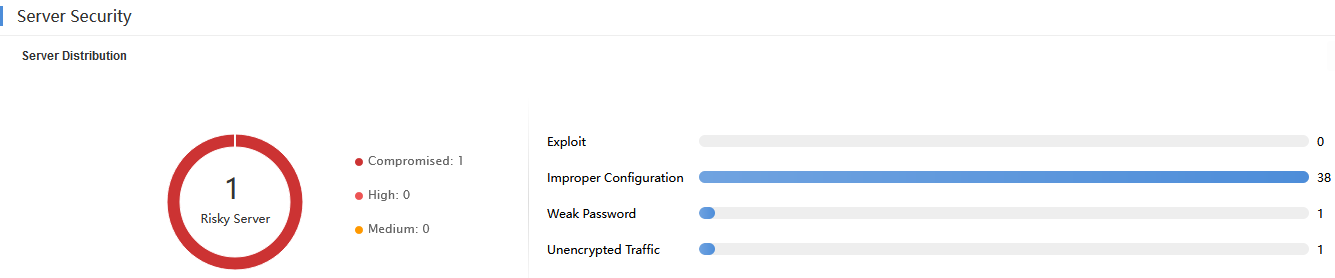
\includegraphics[width=0.9\linewidth]{images/ndr/server-sec.png}
    \caption{Sezione di \emph{Server Security}}
    \label{fig:cc-server-sec}
\end{figure}

\subsection{Host Security}

Durante la scansione dei vari pacchetti, se questi vengono classificati dal sistema come parte di uno scambio malevolo, gli \emph{host} che li hanno inviati o ricevuti vengono segnalati come compromessi. Vengono separati per gravità dell'incidente, come in \autoref{fig:cc-host-sec}.

\begin{figure}[!htbp]
    \centering
    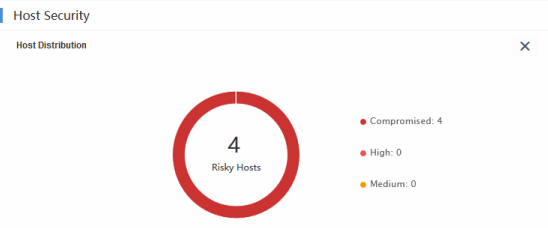
\includegraphics[width=0.8\linewidth]{images/ndr/host-sec-number.png}
    \caption{Sezione di \emph{Host Security}}
    \label{fig:cc-host-sec}
\end{figure}

\section{Segnalazioni}

Il sistema categorizza le segnalazioni in tre livelli di gravità.

\subsection{Incident}

Si tratta di eventi correlati a possibili attacchi. Il CyberCommand mostra anche a quale fase dell'attacco è arrivato. Le fasi mostrate in \autoref{fig:cc-incident} seguono quelle definite nella matrice MITRE ATT\&CK\cite{site:mitre-attck}.

\begin{figure}[!htbp]
    \centering
    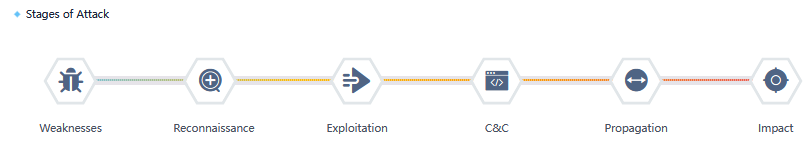
\includegraphics[width=\linewidth]{images/ndr/attack-stage.png}
    \caption{Fasi dell'attacco in una segnalazione \emph{Incident}}
    \label{fig:cc-incident}
\end{figure}

\subsection{Alert}

Si tratta di eventi che non vengono direttamente collegati ad un possibile attacco ma che il sistema considera necessario analizzare perché sospetti.

\subsection{Weakness}

Qui vengono catalogati tutti i problemi rilevati dal sistema. Sono divisi nelle categorie discusse nella \autoref{sec:cc-server-sec}.

\subsection{Analisi del traffico}

La maggior parte degli strumenti di sicurezza di Sangfor si basano su \emph{Neural-X}\cite{site:sangfor-neural-x}, un sistema di analisi \emph{cloud-based} che sfrutta le risorse dei \emph{team} composti da \emph{Data Scientist}, \emph{White Hat Researcher} e \emph{Security Analyst}, insieme ad un sistema di intelligenza artificiale. Questo permette di essere sempre aggiornati sulle ultime minacce e di rilevare anche quelle sconosciute, che non sono ancora state catalogate, tramite l'analisi del comportamento del traffico e dei dispositivi.

Avere uno strumento che riesce a riconoscere in automatico e segnalare il più velocemente possibile ogni minaccia è molto importante, in quanto permette di andare a coprire anche i "punti ciechi" nella rete, dove spesso si notano gli attacchi quando questi sono già in uno stadio avanzato.

Tuttavia, queste analisi devono essere poi raffinate e adattate al contesto specifico in cui vengono utilizzate, in quanto non sempre il comportamento di un dispositivo è malevolo. Ad esempio, un dispositivo che si connette ad un \emph{server} per scaricare un aggiornamento potrebbe essere segnalato come un tentativo di \emph{data exfiltration}, ma in realtà è un comportamento normale e non deve essere segnalato come un problema. Altri esempi sono dispositivi che per loro natura utilizzano protocolli in chiaro e insicuri, per un semplicità e compatibilità, per monitoraggio o test di raggiungibilità. Anche i reparti di sviluppo e test possono essere segnalati come sospetti, in quanto spesso utilizzano ambienti di sviluppo che non rispettano tutte le migliori pratiche di sicurezza, essendo ambienti di test, già racchiusi in una rete sicura e non esposti all'esterno.

\section{Tipologie di problemi rilevati}

Tutti i problemi rilevati dal sistema vengono catalogati come \emph{Alert}, che a loro volta possono scatenare un \emph{Risk}. Quando un dispositivo è legato ad uno o più \emph{Risk}, viene segnalato un \emph{Incident} per indicare una possibile compromissione del determinato \emph{host}.

\subsection{Alert}

Questa tipologia di problemi raccoglie eventi che il sistema non considera attacchi ma che potrebbero essere sospetti. Non vengono mostrati nella \emph{dashboard} principale fino a che non scatenano un \emph{Risk}.

In \autoref{fig:cc-alert-list} possiamo vedere una lista di \emph{Alert}.

\begin{figure}[!htbp]
    \centering
    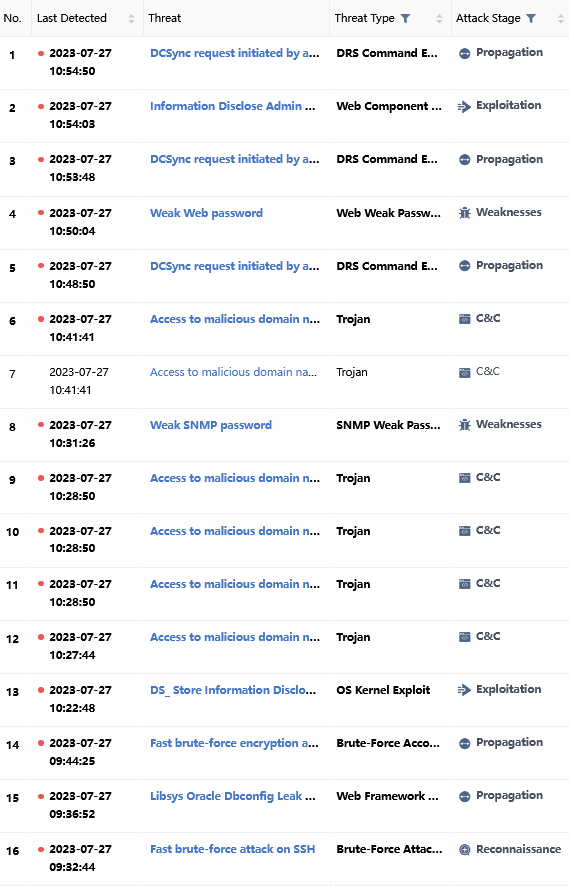
\includegraphics[width=\linewidth]{images/ndr/alert.png}
    \caption{Lista di vari \emph{Alert} rilevati}
    \label{fig:cc-alert-list}
\end{figure}

\subsection{Risk}

In un \emph{Risk} vengono descritti quali problemi sono stati rilevati (\emph{Threat}), la direzione dell'attacco, il punto nelle fasi del MITRE e lo stato attuale, se risolto o meno. Come mostrato in \autoref{fig:cc-risk-detail}, per avere un'idea più precisa è presente un grafico dell'andamento nel tempo e da quale sonda è stata rilevata la minaccia. 

In ottica di integrazione con gli altri strumenti di Sangfor, viene anche segnalata la presenza dell'\emph{Endpoint Secure} sul dispositivo interessato.

\begin{figure}[!htbp]
    \centering
    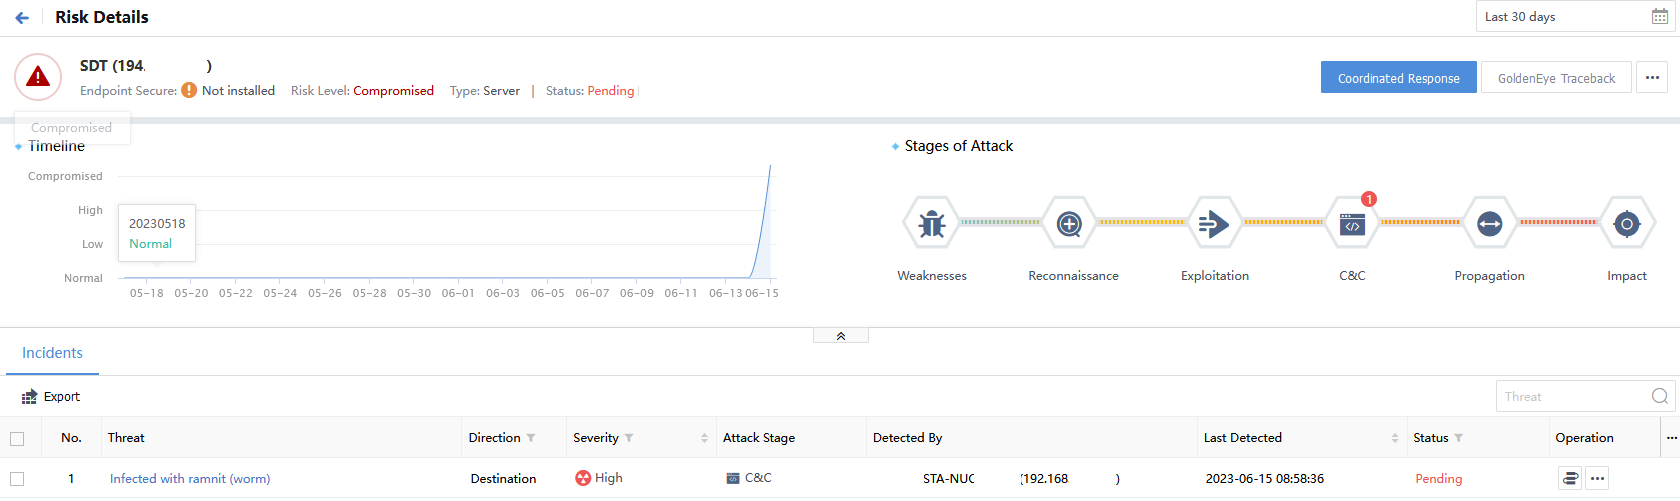
\includegraphics[width=\linewidth]{images/ndr/risk-detail.png}
    \caption{Dettaglio di \emph{Risk}}
    \label{fig:cc-risk-detail}
\end{figure}

\subsection{Incident}

Negli \emph{Incident} vengono raccolti tutti gli attacchi legati un determinato problema, segnalando gli \emph{host} che lo hanno subito e la gravità di esso. 

In \autoref{fig:cc-incident-detail} possiamo vedere un \emph{Incident} legato ad una infezione dovuta ad un \emph{ramnit worm}.

\begin{figure}[!htbp]
    \centering
    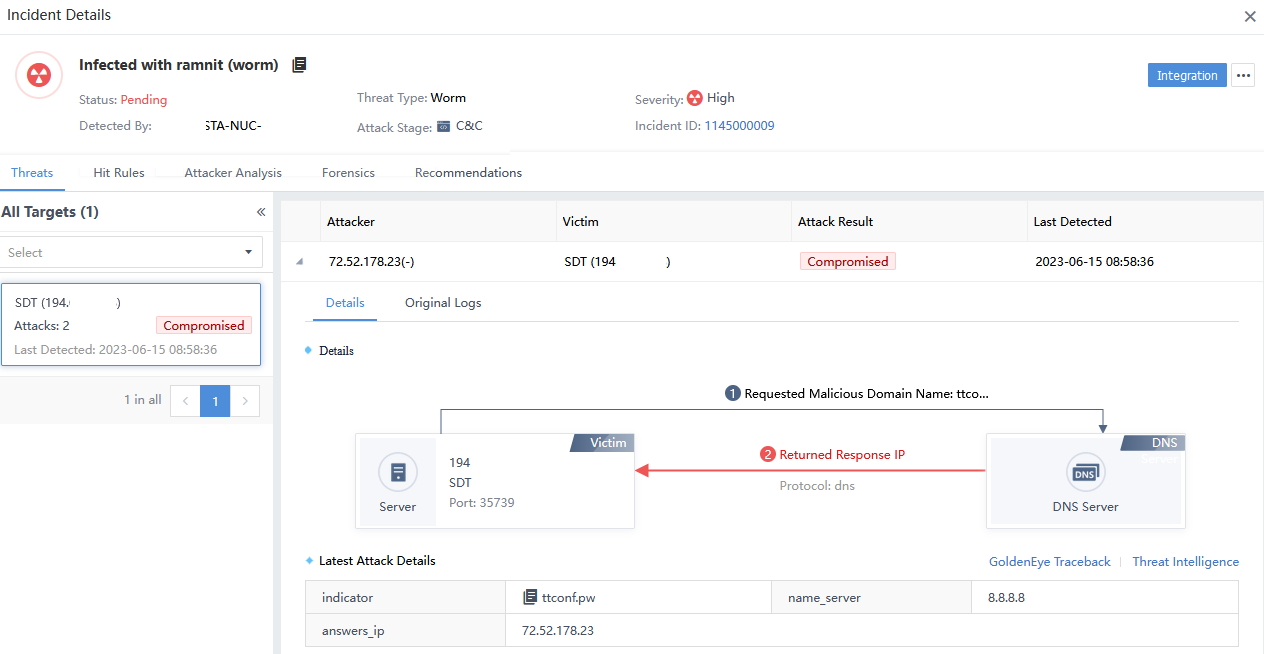
\includegraphics[width=\linewidth]{images/ndr/incident-detail.png}
    \caption{Dettaglio di \emph{Incident}}
    \label{fig:cc-incident-detail}
\end{figure}

Qui ci viene presentato anche un grafico che ci mostra come l'attacco si è propagato, tra quali dispositivi e in che direzione. In questo caso, essendo legato ad una richiesta DNS, vengono mostrati mostrato anche il dominio e i vari IP coinvolti.

\subsection{Flusso di analisi}

Tutto il traffico che le sonde captano viene analizzato solo dopo essere passato attraverso una serie di filtri contenenti una delle \emph{whitelist}, permettendo all'amministratore di sistema di andare a definire cosa non è necessario analizzare. Questo meccanismo è stato utilizzato per evitare di ricevere segnalazioni legate a strumenti che operano per loro natura con protocolli in chiaro, considerati dall'NDR come insicuri, in modo da limitare il numero di falsi positivi. In \autoref{fig:cc-analysis-stream} in che ordine i filtri vengono applicati.

\begin{figure}[!htbp]
    \centering
    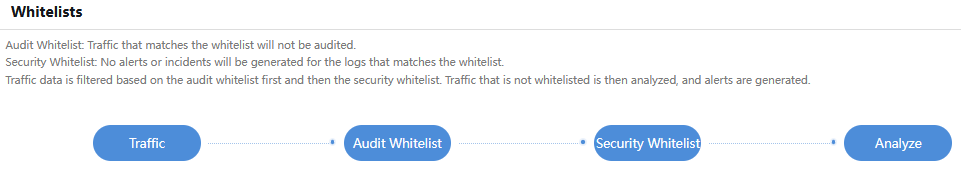
\includegraphics[width=0.9\linewidth]{images/ndr/analysis-stream.png}
    \caption{Flusso di analisi del traffico}
    \label{fig:cc-analysis-stream}
\end{figure}

\subsubsection{Audit Whitelist}

Tramite questa funzionalità tutto il traffico che corrisponde a un certo criterio viene ignorato. Questo è stato utilizzato per evitare di ricevere segnalazioni legate ad esempio a collegamenti noti di cui non era necessario tracciare il traffico, come ad esempio alcune richieste di aggiornamento tra i vari strumenti di monitoraggio verso gli altri dispositivi. Il \emph{form} di definizione di una nuova regola è mostrato in \autoref{fig:cc-audit-whitelist}.

\begin{figure}[!htbp]
    \centering
    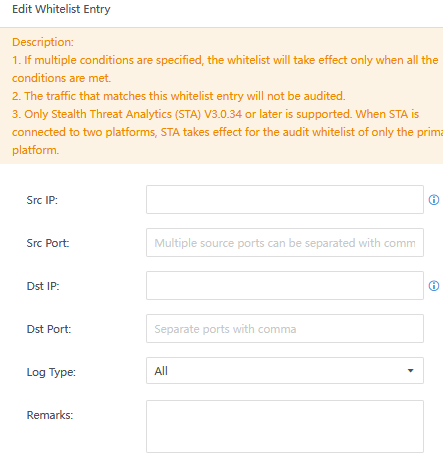
\includegraphics[scale=0.8]{images/ndr/audit-whitelist.png}
    \caption{Definizione di una \emph{Audit Whitelist}}
    \label{fig:cc-audit-whitelist}
\end{figure}

\subsubsection{Security Whitelist}

Tutto il traffico che non viene escluso dalle \emph{Audit Whitelist} passa a questo livello e tutti i \emph{log} che fanno \emph{match} con queste regole non produrranno \emph{Alert} o \emph{Incident}.

\subsubsection{Alert Whitelist}

Permette di specificare quale tipologia di minaccia escludere, indicando sorgenti e destinazioni. È possibile applicarle a gruppi specifici e riferire ai \emph{Rule ID} delle minacce contenute nel database interno del CyberCommand. Il \emph{form} mostrato in \autoref{fig:cc-audit-whitelist} è molto più specifico rispetto a quello delle \emph{Audit Whitelist}.

\begin{figure}[!htbp]
    \centering
    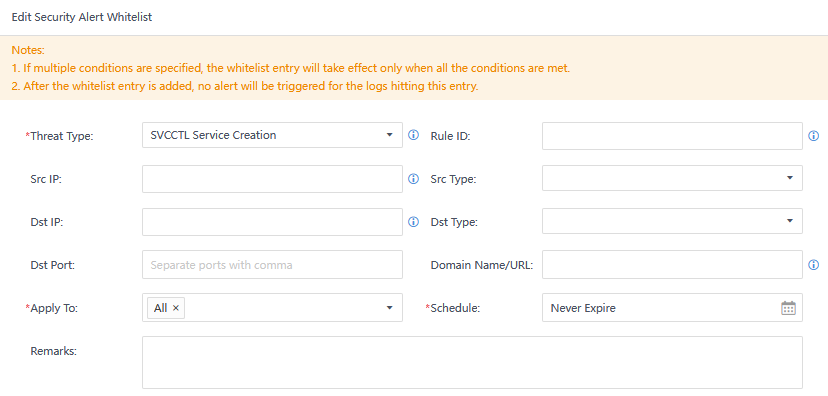
\includegraphics[width=0.8\linewidth]{images/ndr/alert-whitelist.png}
    \caption{Definizione di una \emph{Alert Whitelist}}
    \label{fig:cc-alert-whitelist}
\end{figure}

\subsubsection{Weakness Scan Whitelist}

Permettono di specificare quali rischi escludere dalle segnalazioni, ad esempio per situazioni note o con rischio minimo tale da essere ignorato. Se fatte direttamente dalla scheda di un rischio rilevato è il CyberCommand a consigliare il \emph{Rule ID} di riferimento, ma anche solo con IP/URL e \emph{Risk Type} la regola funziona. La definizione di una \emph{Weakness Scan Whitelist} è mostrata in \autoref{fig:cc-weakness-whitelist}.

\begin{figure}[!htbp]
    \centering
    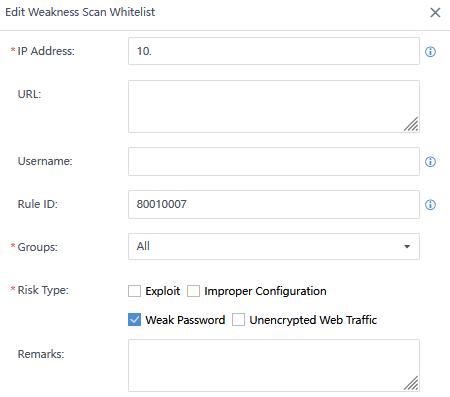
\includegraphics[scale=0.7]{images/ndr/weakness-whitelist.png}
    \caption{Definizione di una \emph{Weakness Scan Whitelist}}
    \label{fig:cc-weakness-whitelist}
\end{figure}

\section{Remediation}

Il CyberCommand permette di configurare delle \emph{remediation}, ovvero una serie azioni in risposta a determinati eventi. Queste possono integrarsi con gli altri strumenti di Sangfor, come \emph{Endpoint Secure} (ES) e \emph{Network Next Generation Firewall} (NGAF). Vengono create tramite uno strumento grafico che permette di definire un diagramma di flusso sfruttando degli elementi preimpostati offerti dal sistema, un esempio è mostrato in \autoref{fig:cc-response-definition}. Le \emph{remediation} possono essere configurate per avviarsi in automatico alla rilevazione di un particolare evento oppure manualmente, in modo da velocizzare la risposta agli eventi più comuni. Verranno discusse nel dettaglio nel capitolo successivo nella \autoref{sec:remediation}.

\begin{figure}[!htbp]
    \centering
    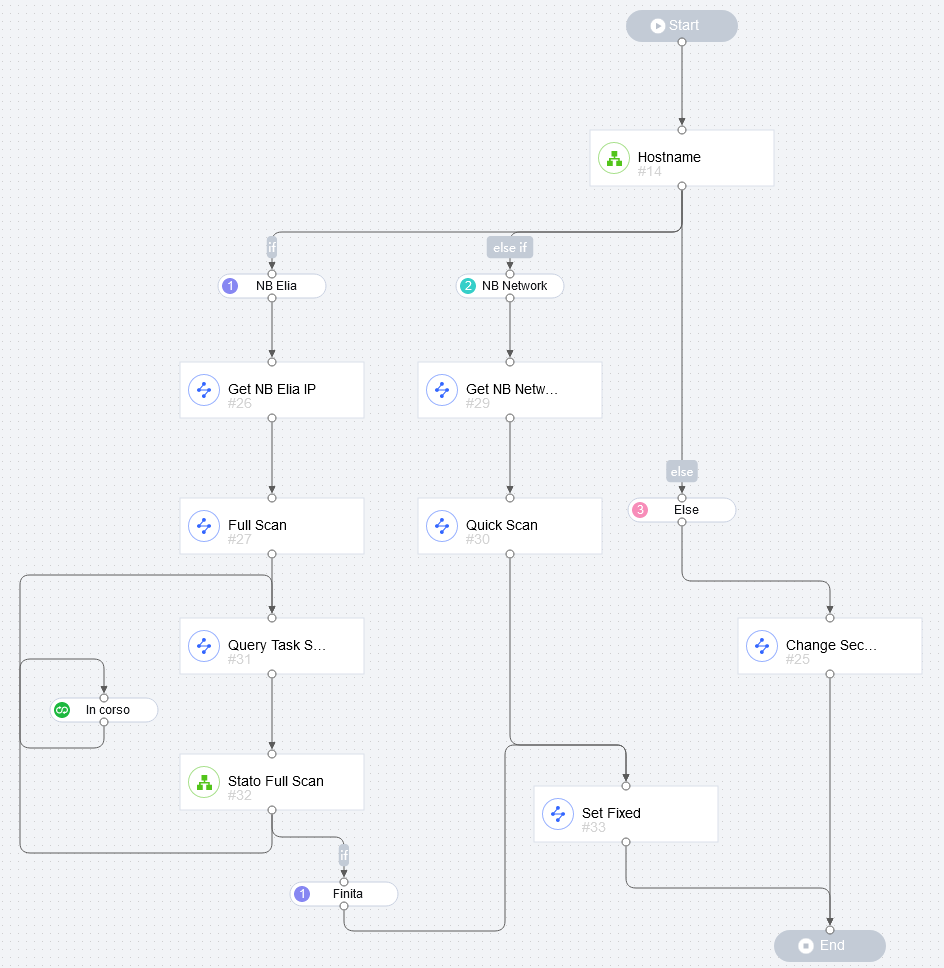
\includegraphics[width=\linewidth]{images/ndr/response.png}
    \caption{Definizione di una \emph{remediation}}
    \label{fig:cc-response-definition}
\end{figure}

I componenti di queste regole di \emph{remediation}, dette \emph{Policy}, sono:

\subsection{Action Node}

Sono i nodi della \emph{policy}, mostrati in \autoref{fig:cc-action-node} dove vengono identificate le azioni da eseguire. Queste sono scelte tra una lista di azioni preimpostate, in base allo strumento che andrà ad eseguirla, ad esempio CyberCommand, \emph{EDR} o altri. Il \emph{Device IP} è sempre quello di chi agisce. Ogni azione ha la possibilità di definire un \emph{delay} di esecuzione per permettere la temporizzazione delle azioni o attesa di altri eventi.

\begin{figure}[!htbp]
    \centering
    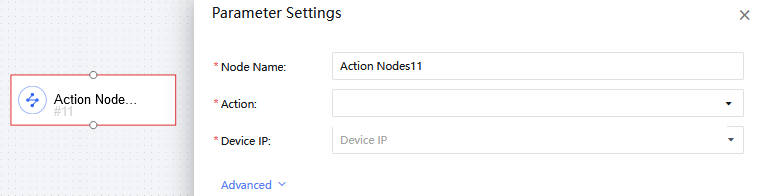
\includegraphics[width=\linewidth]{images/ndr/action-node.png}
    \caption{Elemento \emph{Action Node}}
    \label{fig:cc-action-node}
\end{figure}

\subsection{Decision Node}

Sono i nodi che permettono di prendere decisioni, mostrati in \autoref{fig:cc-decision-node}. Permettono di creare una struttura di \emph{if-then-else} in cui definire vari \emph{branch} da seguire in base a determinate condizioni. I parametri utilizzabili sono definiti internamente dagli strumenti e vengono selezionati tramite un menù a tendina.

Per andare a simulare dei cicli viene utilizzato un sistema di \emph{loopback} che permette di tornare ad un nodo precedente in caso di particolari risultati o condizioni, fino ad un massimo di 10 volte.

\begin{figure}[!htbp]
    \centering
    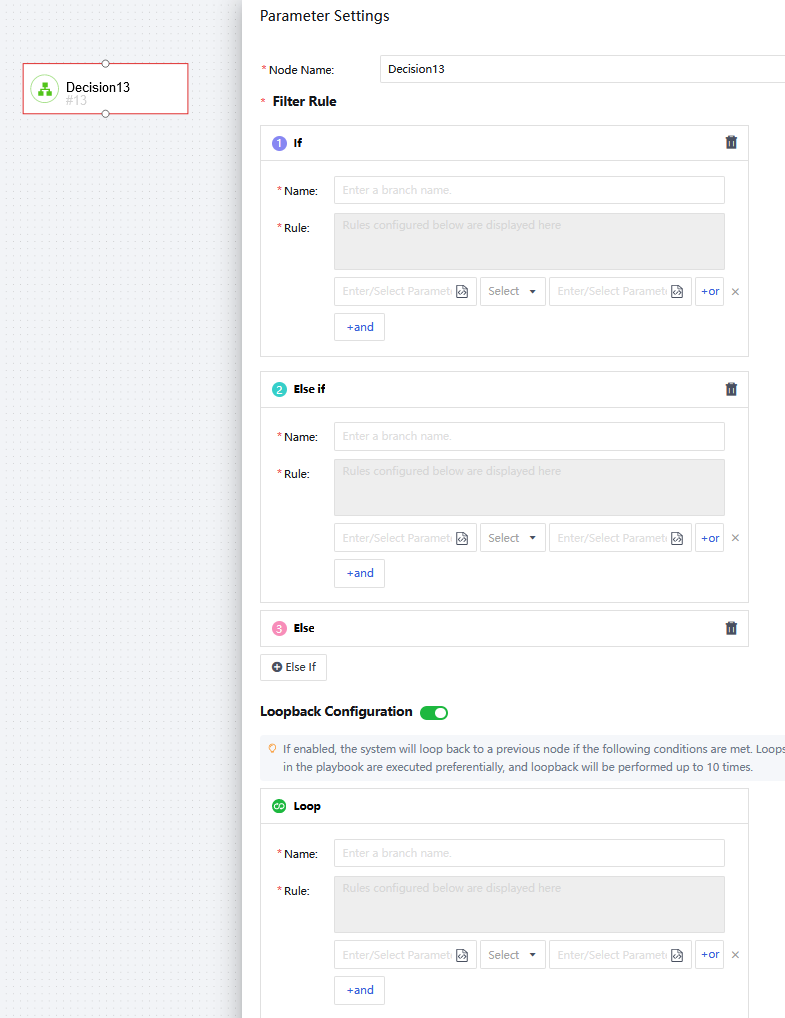
\includegraphics[width=\linewidth]{images/ndr/decision-node.png}
    \caption{Elemento \emph{Decision Node}}
    \label{fig:cc-decision-node}
\end{figure}

\section{Report}

Il CyberCommand permette di generare dei \emph{report}, su richiesta o in automatico, sullo stato della rete, raccogliendo tutti le segnalazioni rilevate, dispositivi coinvolti e azioni intraprese. 

Questi possono essere generati in formato \emph{PDF} e inviati automaticamente via \emph{email}, oppure possono essere consultati direttamente dal sistema.

Possono essere molto utili come supporto per la dimostrazione ai clienti di quanto questo sistema, che lavora silenziosamente in \emph{background}, sia in grado di rilevare e risolvere problemi di sicurezza.